\chapter{State of the art}

%In this chapter, Deep Learning and neural networks are briefly introduced. In addition to that, both the text-to-speech and sentiment analysis tasks are also introduced and discussed, including the challenges that they present as well as the classical and more modern techniques that tackle them, and how they have influenced the development of this project. By the end of this chapter, the core concepts necessary for the discussion of the work done in this publication will have been introduced to the reader.
This chapter gives a brief introduction to the background of this project. The first thing that is discussed is classical methods of speech synthesis, as well as a brief mention of deep learning methods used in this particular task.

Next there is a brief introduction to Deep Learning and deep architectures (both definition and training) a field that is applied to this project. By the end of this chapter, the necessary background will have been introduced for its application in the next chapter.

\section{Speech synthesis}

%Introduction to speech synthesis task
Speech synthesis is the process of generating a synthetic speech signal, emulating that of a real human being. More specifically, this project focuses on synthesizing the signal given text level information. That means, mapping a piece of text to the sounds a human would make to utter said text, and it has to be possible to generate any text that is given to the system.

Speech synthesis has many applications, from medical to recreational. These systems can be used to help speech impaired people and it can also be used to design more human-like interactions objects.

%It can also have beneficial impacts from a more financial perspective, for example, by cheapening the cost of producing audiobooks or other products that require the use of real speech today.&

\subsection{Unit selection}

%Description of the unit selection approach
Unit selection systems render a speech signal by concatenating waveform fragments from a large single-speaker database \cite{hunt1996unit}. The outcome of this technique is highly natural-sounding speech since the fragments that are concatenated come from real waveforms. However, while this system is good at producing natural sounding speech, it lacks the flexibility to produce new speaker sounds or vary the speaking style, as described in \cite{jauk2015creating}, since we are limited by the waveforms database. Each unit also has an associated feature vector containing prosodic information such as pitch and formants.

\begin{comment}
\begin{figure}[h]
    \centering
    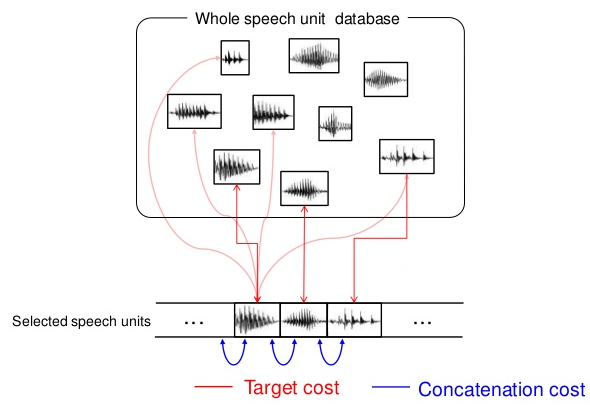
\includegraphics[width=10cm]{figures/unitsel}
    \caption{Unit selection scheme.}
    \label{eq:units}
\end{figure}
\end{comment}

%The best sequence of concatenated units is found by means of dynamic programming using the Viterbi algorithm,  minimizing the cost of concatenating consecutive units. The cost of concatenation is defined in \cite{unit-cost}. Given a sequence of units $u_1^N$, their corresponding prosodic feature vectors $p_1^N$, the total cost of concatenation has two terms:
To choose the best sequence of concatenated units, a cost of concatenation is defined \cite{unit-cost} given a sequence of units $u_1^N = \left \{ u_1, u_2, ..., u_N \right \}$ and their corresponding prosodic vectors $p_1^N$:

\begin{equation}
    C_T^p = C_T^p (u_1^N) = \sum_{i = 1}^{N} C_p (p_t, p_i) 
    \label{eq:pros-cost}
\end{equation}

\begin{equation}
    C_T^c = C_T^c (u_1^N) = \sum_{i = 2}^{N} C_c (u_{i-1}, u_i) 
    \label{eq:concat-cost}
\end{equation}

Where $C_p$ is a function that measures the cost of using a specific feature vector (for example if the units have matching formants and pitch) to match a given target $p_t$ and $C_c$ is the cost of concatenation of two consecutive units (for example a unit ends with the same pitch level that the next one starts with). Finding the best sequence of units is done by using the Viterbi algorithm to minimize the total concatenation cost:

\begin{equation}
    u_1^N= \underset{u_1^N}{argmax} \left \{ \rho \cdot C_T^p (u_1^N) + (1-\rho) \cdot C_T^c (u_1^N) \right \}
    \label{eq:unit-cost}
\end{equation}

\begin{equation}
    0 \le \rho \le 1
\end{equation}

Where $\rho$ is a weighting term that can be used to pay more attention to the targets that to the concatenation, or vice versa.

\subsection{Statistical Parametric Speech Synthesis}

In statistical-parametric speech synthesis (SPSS) a set of spectral and excitation parameters are extracted from a speech corpus from where a set of statistical generative models (typically a hidden Markov model or HMM) are trained to model the them for use in speech synthesis.

\begin{figure}[h]
    \centering
    %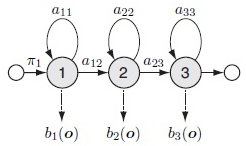
\includegraphics[height=4cm]{figures/hmm}

    \tikzstyle{vertex}=[draw,black,fill=blue,circle,minimum size=24pt,inner sep=0pt]
\tikzstyle{edge}=[very thick]
\begin{tikzpicture}[scale=2.5]
    \node (a)[vertex,fill=gray!10,align=left] at (0,0) {$1$};
    \node (b)[vertex,fill=gray!10,align=left] at (1,0)  {$2$};
    \node (c)[vertex,fill=gray!10,align=left] at (2,0)  {$3$};
    \node (pi1) at (-0.5,0.5) {$\pi_1$};
    \node (pi2) at (0.5,0.5) {$\pi_2$};
    \node (pi3) at (1.5,0.5) {$\pi_3$};
    \node (b1) at (0,-0.35) {$b_1$};
    \node (b2) at (1,-0.35) {$b_2$};
    \node (b3) at (2,-0.35) {$b_3$};
    \path[thick,->] (a)    edge node [anchor=center,above,sloped] {$a_{1 \rightarrow 2}$} (b);
    \path[thick,->] (b)    edge node [anchor=center,above,sloped] {$a_{2 \rightarrow 3}$} (c);
    \path[thick,->] (a)    edge[loop above, looseness=10] node [anchor=center,above,sloped] {$a_{1 \rightarrow 1}$} (a);
    \path[thick,->] (b)    edge[loop above, looseness=10] node [anchor=center,above,sloped] {$a_{2 \rightarrow 2}$} (b);
    \path[thick,->] (c)    edge[loop above, looseness=10] node [anchor=center,above,sloped] {$a_{3 \rightarrow 3}$} (c);
    \path[thick,->] (pi1)  edge[looseness=1] node [anchor=center,above,sloped] {} (a);
    \path[thick,->] (pi2)  edge[looseness=1] node [anchor=center,above,sloped] {} (b);
    \path[thick,->] (pi3)  edge[looseness=1] node [sloped] {} (c);
\end{tikzpicture}


    \caption{A 3-state left-to-right Hidden Markov Model.}
    \label{fig:hmm}
\end{figure}

As seen in Figure \ref{fig:hmm}, a HMM is a finite state machine that can be described by the tuple $\lambda = \left < A, B, \Pi \right >$ where $A$ are the state transition probabilities, $B$ are the output distributions on each state (spectral \& excitation output parameters) and $\Pi$ are the initial state probabilities. HMMs provide a time-discrete series of observations from a distribution of the speech parameters. In contrast with unit selection, SPSS models offer a more compact representation than unit selection since they don't require a large database after the models have been trained.

\begin{figure}
    \centering
    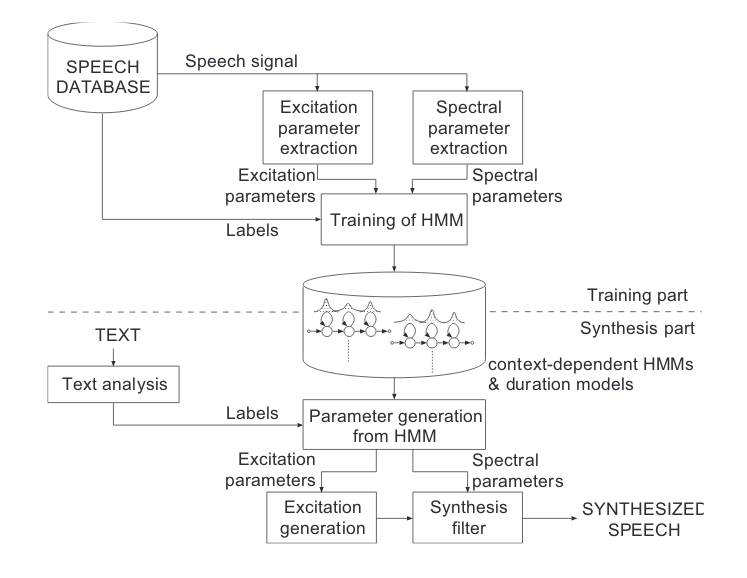
\includegraphics[height=12cm]{figures/hts}
    \caption{SPSS system based on HMMs. This scheme corresponds to the HTS framework \cite{zen2007hmm}.}
    \label{fig:hts}
\end{figure}

Moreover, SPSS also overcomes the limitation of only being limited to one speaker, since we can easily modify the speaker characteristics and speaking styles by transforming the model parameters appropriately as describes in \cite{zen2007hmm} and \cite{pascual2006deep}.

%In the methodology chapter of this document, the concepts from this section will be revisited and explained more in-depth.

\subsection{Recurrent Neural Network-based Speech Synthesis} \label{sec:rnn-tts}

%RNNs
Another approach to speech synthesis more closely related to this project, is using recurrent neural networks (RNNs) to process a sequence of linguistic features and predict the same excitation and spectral parameters from SPSS.

RNNs are covered in more detail in a later section of this chapter. As describes by \cite{chen1998rnn}, this scheme consists of using neural networks to generate parametric speech in two stages: a duration model that predicts the duration of a phoneme in a sentence, and an acoustic model to predict the spectral and excitation parameters for as many time steps as predicted by the duration model. Figure \ref{fig:rnn-tts-0} shows the complete scheme of this approach.

\begin{figure}[h]
\centering
    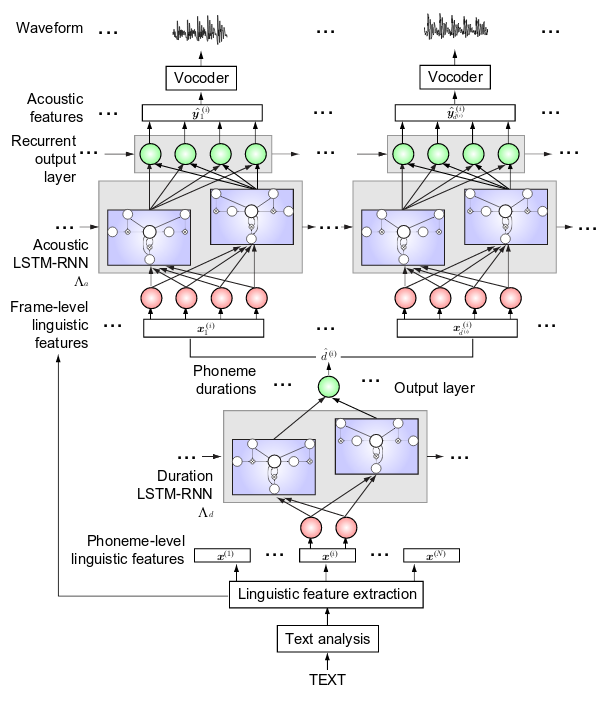
\includegraphics[height=13cm]{figures/rnn-tts}
    \caption{RNN-based SPSS scheme. Concepts such as LSTM that appear in the figure are covered at later section of this chapter. The figure is originally from \cite{chen1998rnn}}
    \label{fig:rnn-tts-0}
\end{figure}

\subsection{Expressive speech synthesis}

%Summary of the bibliography of the approaches to expressive speech synthesis.
%Expressive speech synthesis
The techniques from the previous sections for doing speech synthesis typically only offer a single speaking style that is independent of the message that is being transmitted. In \cite{bulut2002expressive} and \cite{eide2004corpus} a prosodic target is modeled in order to synthesize a text with different types of emotions using a unit selection systems and pitch prediction to modify the prosodic content of the speech.

More recently, \cite{jauk2016acoustic} uses deep neural networks (more on this in the following sections) to predict acoustic features of expressive speech from semantic vector space representations. The results can be used to enhance the inputs of speech synthesis systems by modeling the expressiveness of a corpus in SPSS systems, which in contrast with \cite{bulut2002expressive} and \cite{eide2004corpus}, the synthesis would adapt to the semantic content of the message.

\section{Text classification for sentiment Analysis}

Text classification is a task in natural language processing \cite{chowdhury2003natural} (NLP) where a text is assigned a given label automatically. A classic model used for text classification is bag of words \cite{wallach2006topic} (BOW), where a piece of text is assumed to be a sequence of words picked at random from a specific set. In the topic of text classification, classifying text using BOW would involve predicting the set the text belongs to (for example, a SPAM email contains specific words common to all SPAM emails, or a positive text may contain words that are different from a negative text).

More recently, more modern techniques such as deep learning have been used to improve the accuracy of these systems. In \cite{zhang2015character} text is treated as a signal an processed using Convolutional neural networks (more on this in the next sections) and \cite{DBLP:journals/corr/Kim14f} uses vector representations of words (word embeddings \cite{goldberg2014word2vec}) to classify text.

%Introduction to the sentiment or text classification task.

\section{Deep Learning} \label{sec:dnn}

In recent years, deep structured learning, or more commonly called deep learning is a set of techniques that has risen in popularity and established itself as a new area of machine learning among the scientific and research communities. \cite{deng2014deep}

\cite{bengio2009learning} discussed the limitations of shallow architectures and provided a theoretical basis to the advantages of deeper ones. But it has only been in recent years that such architectures have been able to be put into production with ever-growing popularity thanks to compute technologies being every time more available and affordable to consumers.

With deep learning architectures, it is possible to learn complex non-linear representations from large amounts of data. Raw data can be processed and turned into several levels of higher level representations to make it possible to reason about it and make tasks such as classification easier and more effective.

In addition to more compute power, large datasets that can take advantage of deep models such Imagenet \cite{russakovsky2015imagenet} are being made publicly available. These datasets are often used as benchmarks and serve as points of reference to drive research and development forward.

%In summary, one could describe Deep Learning as models capable of obtaining high level information from low level one, and the compute resources and databases that make training of these models possible.

\subsection{Deep Neural Networks}

In Deep Learning, a common architecture is the so called Deep Neural Network (DNN), which is an artificial neural network with a large number of hidden layers. The desire to decomposing a signal into higher levels of abstraction drives such neural networks configurations, and since more layers require more trainable parameters, large amounts of training data are also needed to train them.

\begin{figure}[h]
    \centering
    \scalebox{.75} { \begin{tikzpicture}[
init/.style={
  draw,
  circle,
  inner sep=2pt,
  font=\Huge,
  join = by -latex
},
squa/.style={
  draw,
  inner sep=2pt,
  font=\Large,
  join = by -latex
},
start chain=2,node distance=13mm
]
\node[on chain=2] 
  (x2) {$x_2$};
\node[on chain=2,join=by o-latex] 
  {$w_2$};
\node[on chain=2,init] (sigma) 
  {$\displaystyle\Sigma$};
\node[on chain=2,squa,label=above:{\parbox{2cm}{\centering Activate \\ function}}]   
  {$f$};
\node[on chain=2,label=above:Output,join=by -latex] 
  {$y$};
\begin{scope}[start chain=1]
\node[on chain=1] at (0,1.5cm) 
  (x1) {$x_1$};
\node[on chain=1,join=by o-latex] 
  (w1) {$w_1$};
\end{scope}
\begin{scope}[start chain=3]
\node[on chain=3] at (0,-1.5cm) 
  (x3) {$x_3$};
\node[on chain=3,label=below:Weights,join=by o-latex] 
  (w3) {$w_3$};
\end{scope}
\node[label=above:\parbox{2cm}{\centering Bias \\ $b$}] at (sigma|-w1) (b) {};

\draw[-latex] (w1) -- (sigma);
\draw[-latex] (w3) -- (sigma);
\draw[o-latex] (b) -- (sigma);

\draw[decorate,decoration={brace,mirror}] (x1.north west) -- node[left=10pt] {Inputs} (x3.south west);
\end{tikzpicture}
 }
    \scalebox{.5} { \begin{tikzpicture}[
plain/.style={
  draw=none,
  fill=none,
  },
net/.style={
  matrix of nodes,
  nodes={
    draw,
    circle,
    inner sep=10pt
    },
  nodes in empty cells,
  column sep=2cm,
  row sep=-9pt
  },
>=latex
]
\matrix[net] (mat)
{
|[plain]| \parbox{1.3cm}{\centering Input\\layer} & |[plain]| \parbox{1.3cm}{\centering Hidden\\layer} & |[plain]| \parbox{1.3cm}{\centering Output\\layer} \\
& |[plain]| \\
|[plain]| & \\
& |[plain]| \\
  |[plain]| & |[plain]| \\
& & \\
  |[plain]| & |[plain]| \\
& |[plain]| \\
  |[plain]| & \\
& |[plain]| \\    };
\foreach \ai [count=\mi ]in {2,4,...,10}
  \draw[<-] (mat-\ai-1) -- node[above] {Input \mi} +(-2cm,0);
\foreach \ai in {2,4,...,10}
{\foreach \aii in {3,6,9}
  \draw[->] (mat-\ai-1) -- (mat-\aii-2);
}
\foreach \ai in {3,6,9}
  \draw[->] (mat-\ai-2) -- (mat-6-3);
\draw[->] (mat-6-3) -- node[above] {Ouput} +(2cm,0);
\end{tikzpicture}
 }
    %\caption{Neural network basic configuration. Each layer consists of a net of nodes chich perform a linear operation of the inputs, before being fed to an activation function at the output and fed to the next layer.}
    \caption{Basic neuron (left) and neural network configuration (right).}
    \label{fig:neural-net}
\end{figure}

DNNs are defined by stacking several layers of basic units called neurons. In each layer, a linear operation takes place, where the inputs $\mathbf{x}= \left \{ 1, x_1, x_2, ..., x_N \right \}$ ($1$ is for a bias term) are linearly combined by a set of weights that are characteristic of each layer. The output of this linear operation is fed to a non-linear activation function (such as a sigmoid (\ref{eq:sigmoid}) or a tanh) which introduces the non-linearities of the system. Equation \ref{eq:neural-layer} shows the operation that takes place in the $i$-th layer, where $\mathbf{W_i}$  is the matrix of weights, $\mathbf{x_i}$ is the input vector of the layer, $\mathbf{y_i}$ is the output vector and $\sigma$ is the activation function.

\begin{equation}
    \centering
    \mathbf{y_i} = \sigma \left ( \mathbf{W_i} \cdot \mathbf{x_i} \right )
    \label{eq:neural-layer}
\end{equation}

\begin{equation}
    \centering
    \sigma (x) = \frac{1}{1 + e^{-x}} 
    \label{eq:sigmoid}
\end{equation}

The outputs of this activation function are fed to the next layer of neurons until the last layer of a network, typically a softmax activation function for classification tasks or linear operation in regression ones. Figure \ref{fig:neural-net} shows a neural network configuration.

\subsection{Optimization}

%Back propagation algorithm and optimizers.
Optimizing, or training, a DNN is the process of finding the best possible set of weights that accomplish the best results in a given task. A task that DNNs are used for is classification, where a label is assigned to each input vector (predicting wether an image is from a cat or a dog) and also regression (predicting the expected cost of a property given the land size and proximity to the coast).

To optimize the network a cost or loss function is defined to measure the error of the predictions (such as the root mean square error or the cross-entropy error \cite{golik2013cross}). given a loss, we can improve the performance of a model by translating the weight vector in the direction of the gradient.

\begin{equation}
    L(\mathbf{x}; \mathbf{w}) = \sum_{\mathbf{x}_k}^{} L (\mathbf{x_k})
    \label{eq:loss}
\end{equation}

\begin{equation}
    w_i[n+1] = w_i[n] - \lambda \frac{\partial L(\mathbf{x}; \mathbf{w}[n])}{\partial w_i}
    \label{eq:update_w}
\end{equation}

Equation \ref{eq:loss} is a loss function, computed by adding the errors of a batch of vectors of a dataset. These vectors are the examples from where the network learns. The size of the batch is usually fixed and smaller than the total size of the dataset, and is used to perform an iteration in the weight update process (Equation \ref{eq:update_w}). This technique is called stochastic gradient descent \cite{bottou2010large} (SGD).

Before updating the weights, the partial derivatives of the loss function are computed using the back-propagation algorithm \cite{chauvin1995backpropagation}. For this we need to be able to compute the derivatives of both the loss function and the activation functions of the neurons, and the update is performed like in Equation \ref{eq:update_w}.

The norm of the gradient can be scaled by a factor called learning rate (expressed as $\lambda$ in Equation \ref{eq:update_w}) to speed-up or slow-down the convergence of the loss function during training. Ways to improve this weight updates are Adam \cite{kingma2014adam} and Adadelta \cite{zeiler2012adadelta}.

%\begin{figure}
%    \centering
%    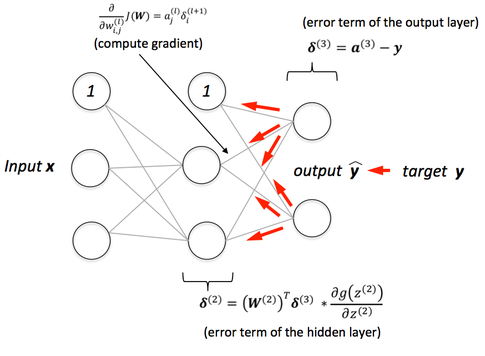
\includegraphics[height=6cm]{figures/backpropagation}
%    \caption{back propagation}
%    \label{fig:back-prop}
%\end{figure}

%To obtain the gradients of the loss function with respect to the weights, the back-propagation algorithm \cite{chauvin1995backpropagation} is used to compute them analytically. This algorithm computes the partial derivatives of the loss function with respect to the weights, given the partial derivatives of the layers later layers, hence the name back-propagation. For this to work, the loss function has to be diferentiable and for this to be true the activation functions of the hidden layers also have to be as well.

%Equation \ref{eq:loss} implies that the loss can be computed given a batch of input vectors, thus the weight updates happen after the network has processed a collection of inputs. We don't need however to process an entire dataset and only use a small portion of it before the update step, in a techniche called stochastic gradient descent (SGD) \cite{bottou2010large}.

\section{Recurrent networks}

%Introductio to RNNs. How they are trained and introduction of the vanishing/exploding gradient.
Recurrent neural networks (RNN) are a special type of architecture capable of modeling sequences, where the outputs of a hidden layer are fed back to the inputs of the same layer. This feedback loop introduces a state in the neurons and the output of the layers can be rewritten as:

\begin{equation}
    \centering
    \mathbf{y_t} = \sigma \left ( \mathbf{W} \cdot \mathbf{x_t} + \mathbf{U} \cdot \mathbf{y_{t-1}} \right )
    \label{eq:out-rec}
\end{equation}

Where $\mathbf{x_t}$ is an input vector at the $t$-th timestep and $\mathbf{U}$ is an additional matrix of tranable weights. Because of the introduction of a neuron state, RNNs can model various types of sequential data (predict the next frame of a video given the N first, translate a sequence of words to another a different language, predict the duration of each of the phonemes in a sequence, etc...).

Recurrent networks can still be trained efficiently by using back-propagation through time \cite{werbos1990backpropagation} which is specific case of back-propagation where the errors are also back-propagation back in time. If we expand \ref{eq:out-rec} we get:

\begin{figure}
    \centering
    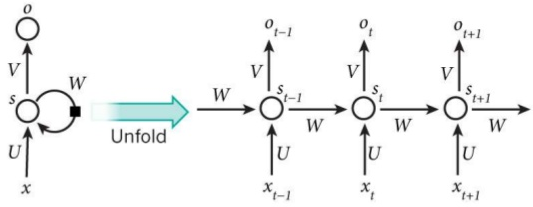
\includegraphics[height=4cm]{figures/unfold}
    \caption{Unfolded RNN}
    \label{fig:unfold}
\end{figure}

\begin{equation}
    \centering
    \mathbf{y_t} = \sigma \left ( \mathbf{W} \cdot \mathbf{x_t} + \mathbf{U} \cdot \sigma \left ( \mathbf{W} \cdot \mathbf{x_{t-1}} + \mathbf{U} \cdot \sigma \left ( \cdots \sigma \left ( \cdots \right ) \cdots \right ) \right ) \right )
    \label{eq:out-rec-expanded}
\end{equation}

The recursive multiplication of $U_t$ make RNNs a special case of DNNs, where the repeated multiplications can cause the gradients to become too small or too big by the time they reach the inputs of the network when doing back-propagation. This is due to the vanishing or exploding gradient problem \cite{bengio1994learning} that occurs in SGD.

To mitigate this problem in RNNs, we can use specially designed recurrent neurons such as Long Short-Term Memory as opposed to regular RNNs.

\subsection{Long Short-Term Memory (LSTM)}

Long Short-Term Memory \cite{hochreiter1997long} or LSTM are a special kind of recurrent unit that deals with the aforementioned problem of the vanishing gradient. This cell works by introducing gating mechanism operated by soft switches trained while optimizing the network that control the flow of information coming in and out of the cell.

\begin{comment}
\begin{figure}[h]
    \centering
    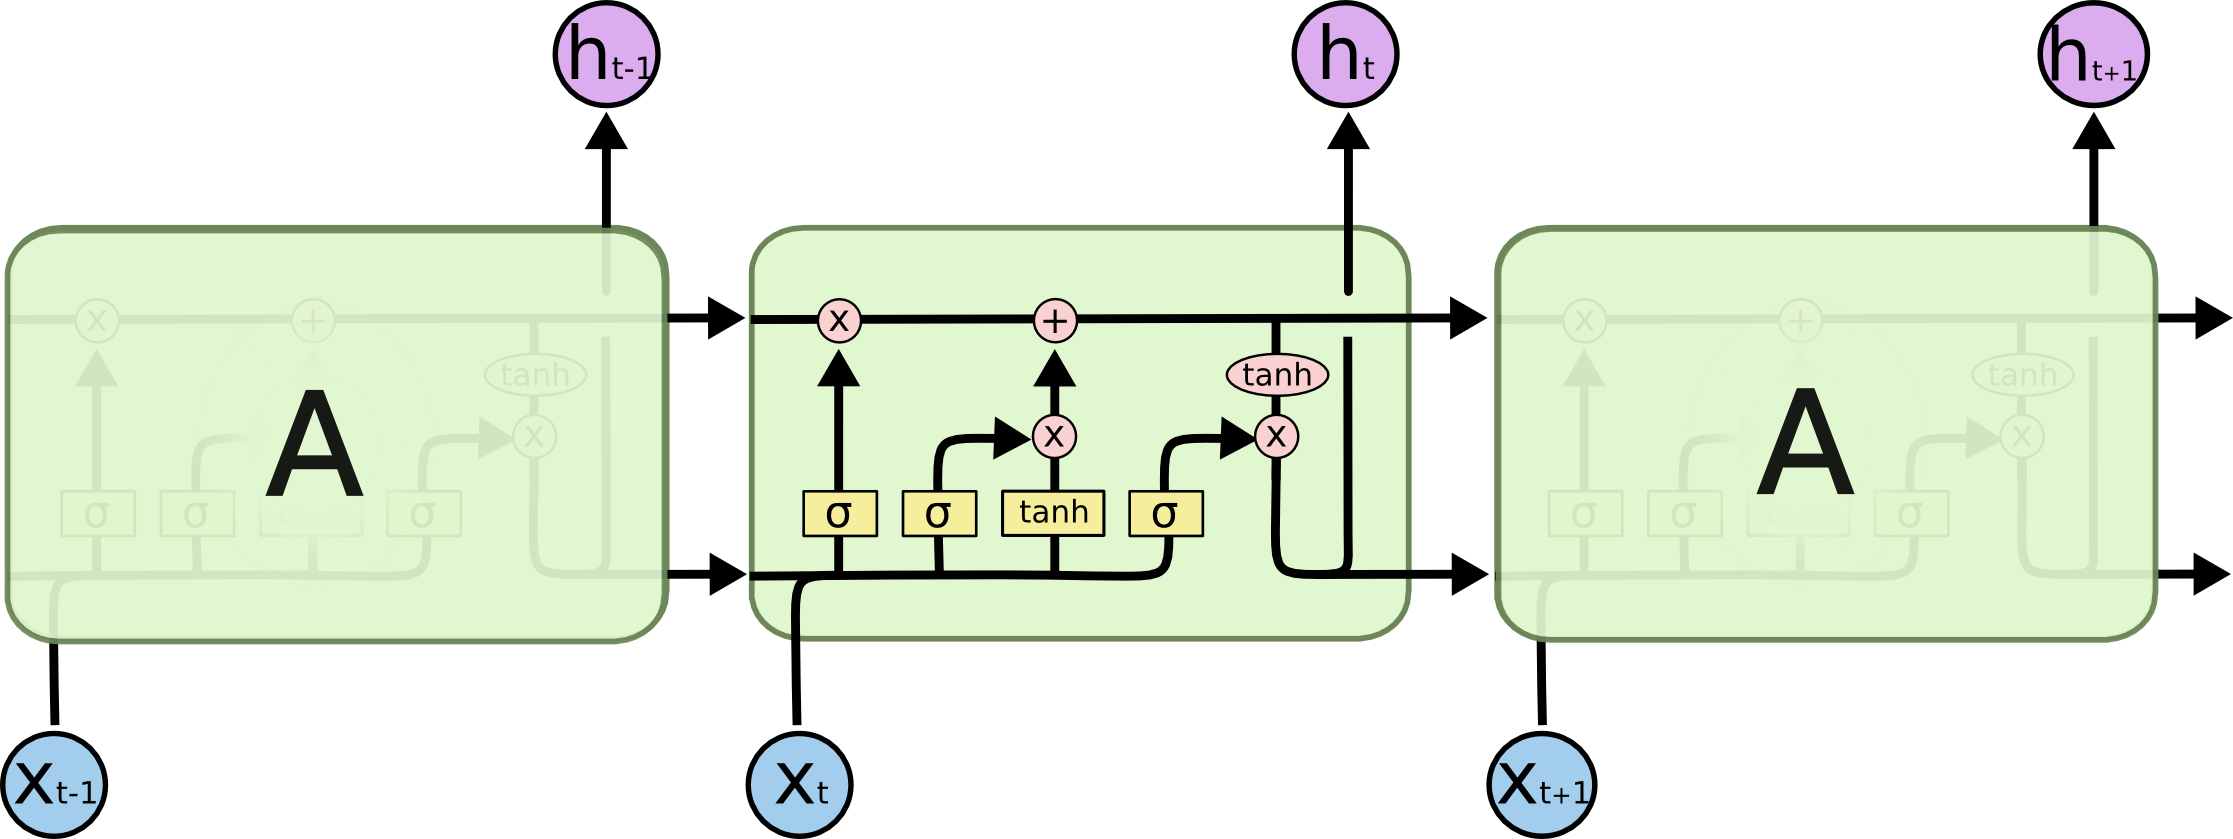
\includegraphics[height=4cm]{figures/lstm-chain}
    \caption{Diagram of a chain of LSTM units. The horizontal axis represents time and the vertical represents the RNN-LSTM at each time step. $X_t$ are the input vectors at the past, present and future time step. The gating mechanism controls the flow of information that is input to the next state of the layer. This figure was taken from \cite{lstm}}
    \label{fig:lstm}
\end{figure}
\end{comment}

\section{Convolutional Neural Networks}

As seen in Equation \ref{eq:neural-layer}, a neuron activation depends on all the output activation of the previous layer. Convolutional neural networks (CNN) are a type of architecture that contain a type of hidden layers called Convolutional layers. These architectures have proven to be very effective in computer vision applications but they are also used with success in NLP tasks \cite{zhang2015character}.

Rather than combining all the outputs of the previous layer, CNN neurons only focus on the activations of a fixed number of neurons from the previous layer \cite{krizhevsky2012imagenet}. While each neuron focuses on a different set of inputs, the total number is fixed and the weights are shared among the activations of the layer. Because of this, we can think of these layers as having an associated kernel that is used to filter the previous layer by means of a convolution to produce a feature map in the layer. The number of feature maps is a parameter of the convolutional layer. %By stacking these layers, the deepest layers can learn very speciliced filters from low level features learnt in the earlier layers (for example a filter that detects faces in a picture, deppends on a filter that detects straight and round edges), making these architectures very popular in computer vision tasks.

